% =============================================================================
% PESSOA 2 — SEÇÃO 3.2 (POWER ANALYSIS & FAILURE MODES) & SEÇÃO 4 (LIMITATIONS)
% Padrão: ACM sigconf (\documentclass[sigconf]{acmart})
% Contém versão em Inglês (padrão ACM/ACL) e versão em Português logo abaixo.
% Compatível com o arquivo unificado: paper/references.bib
% =============================================================================

% -----------------------------------------------------------------------------
% [VERSÃO 1: INGLÊS — PADRÃO ACM SIGCONF]
% -----------------------------------------------------------------------------

\subsection{Statistical Power Audit \& Tokenization Failure Modes}
\label{sec:power_and_failures}

Showing that downstream differences are statistically indistinguishable from zero (p>0.05) does not prove equivalence unless the evaluation possesses sufficient statistical power to detect meaningful regressions. Following Miller (Section~5)~\cite{miller2024adding} and cluster-inference theory~\cite{abadie2022when}, we compute the Minimum Detectable Effect (MDE) at $80\%$ power (1-=0.80,z0.80=0.842) and two-sided =0.05 (z0.975=1.960), along with the required sample size Nreq to detect a target accuracy drop :
\begin{equation}
\mathrm{MDE} = (z_{1-\alpha/2} + z_{1-\beta})\,\mathrm{SE}_{A-B,\mathrm{clustered}}, \quad
N_{\mathrm{req}}(\Delta) = \frac{2(z_{1-\alpha/2} + z_{1-\beta})^2 (1-\rho)\,p(1-p)\,\mathrm{DEFF}}{\Delta^2}.
\label{eq:mde_power}
\end{equation}

\begin{figure}[t]
    \centering
    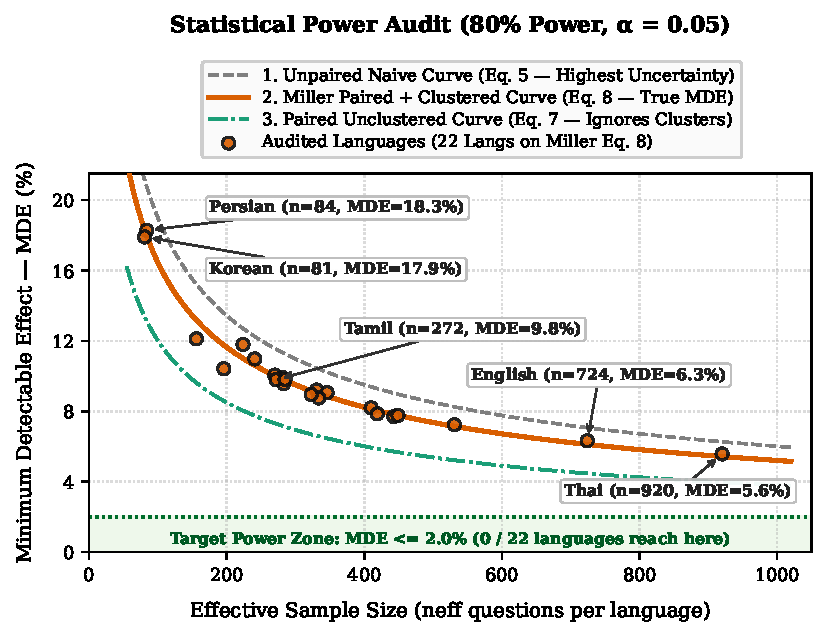
\includegraphics[width=\columnwidth]{figures/fig2_power_mde.pdf}
    \vspace{-1.5em}
    \caption{Minimum Detectable Effect (MDE) at $80\%$ power (=0.05) as a function of effective sample size neff. Overlaying the 22 languages from Table~2 of~\cite{foroutan2026parity} reveals that \textbf{0 out of 22 languages} reach the adequate power zone ($\mathrm{MDE} \le 2.0\%$).}
    \label{fig:power_mde}
    \vspace{-1.0em}
\end{figure}

\textbf{Severe Under-Powering Across Languages:} Figure~\ref{fig:power_mde} demonstrates that \textbf{22 out of 22 languages ($100\%$)} are statistically underpowered to detect a $1.0\%$ or $2.0\%$ accuracy degradation. Across all 22 languages, the mean MDE is $\pm 11.38\%$ under naive unpaired errors (Eq.~5 of~\cite{miller2024adding}), drops to $\pm 7.22\%$ with question-level pairing (Eq.~7), and rebounds to $\mathbf{\pm 9.88\%}$ under Miller's paired-and-clustered estimator (Eq.~8). Even the highest-coverage languages---Thai ($n_{\mathrm{eff}} = 920, \mathrm{MDE} = \pm 5.58\%$) and English ($n_{\mathrm{eff}} = 724, \mathrm{MDE} = \pm 6.27\%$)---cannot reliably detect drops smaller than $5.5\%$. For single-benchmark languages such as Korean ($n_{\mathrm{eff}} = 81, \mathrm{MDE} = \pm 17.75\%$) and Persian ($n_{\mathrm{eff}} = 84, \mathrm{MDE} = \pm 18.29\%$), the evaluation is blind to regressions of up to 18 percentage points. In the 22-language global aggregate, cross-lingual clustering across parallel benchmarks~\cite{nllb2022no} inflates the global MDE from $\pm 1.60\%$ to $\mathbf{\pm 4.48\%}$. Consequently, actual statistical power across languages averages just $6.2\%$ for a $1.0\%$ drop and $9.7\%$ for a $2.0\%$ drop; achieving $\mathrm{MDE} \le 2.0\%$ requires an average of Nreq=6,723 clustered questions per language (26.8 the current benchmark size).

\begin{table}[t]
\centering
\caption{Algorithmic failure modes of Parity-Aware BPE (Hybrid Fair-Max)~\cite{foroutan2026parity} vs.\ Classical BPE under \texttt{Whitespace()} pre-tokenization. Phase-1 global merges preserve common tokens, whereas Phase-2 \textit{fair-max} reallocation fragments high-resource long-tail morphemes and digits.}
\vspace{-0.6em}
\footnotesize
\setlength{\tabcolsep}{2.8pt}
\begin{tabular}{lcccc}
\toprule
\textbf{Domain / Failure Mode} & \textbf{Classical} & \textbf{PA-Hybrid} & \textbf{Ratio} & \textbf{Overhead} \\
\midrule
Code Syntax (Python)       & 16 & 26 & 1.62 & $+62.5\%$  \\
Mathematical / Numeric     & 19 & 37 & 1.95 & $+94.7\%$  \\
Structured JSON / API      & 23 & 52 & 2.26 & $+126.1\%$ \\
German Compound Nouns      & 12 & 35 & 2.92 & $+191.7\%$ \\
English STEM Terminology   & 10 & 43 & 4.30 & $+330.0\%$ \\
\bottomrule
\end{tabular}
\vspace{-0.8em}
\label{tab:failure_modes}
\end{table}

\textbf{Tokenization Failure Modes in Specialized Domains:} To understand where PA-BPE's compression loss manifests structurally, we execute both Classical BPE and Hybrid PA-BPE (\textit{fair-max}, Eq.~6 of~\cite{foroutan2026parity}) with the official \texttt{Whitespace()} pre-tokenizer across five technical domains (Table~\ref{tab:failure_modes}). While Phase-1 global merges preserve top-frequency keywords (\texttt{def}, \texttt{return}, \texttt{and}, \texttt{und}), Phase-2 reallocates tail merges toward low-resource scripts (Tamil, Telugu, Korean, Persian), inducing severe over-segmentation in structured inputs:
\begin{itemize}
    \item \textbf{Code \& Structured JSON ($+62.5\%$ to $+126.1\%$ overhead):} Domain identifiers (\texttt{calculate}  \texttt{c|al|c|ul|at|e}) and JSON schema keys/enums (\texttt{transaction}, \texttt{PENDING\_VERIFICATION}) shatter into character fragments, inflating KV-cache memory and structured decoding latency~\cite{petrov2023language,ahia2023all}.
    \item \textbf{Numbers \& Arithmetic (1.95 tokens):} Classical BPE consolidates recurring 3-digit blocks (\texttt{141|592|653}), whereas PA-BPE fragments decimal mantissas into single and paired digits (\texttt{1|4|1|59|2...}), impairing positional alignment in multi-digit arithmetic~\cite{singh2024tokenization}.
    \item \textbf{German Compounds \& STEM (2.92 to 4.30 tokens):} Productive German compound roots (\texttt{schiff|fahrts}  \texttt{sch|if|f|f|a|h|r|ts}) and Latin/Greek STEM morphemes (\texttt{neuro|degenerative}  12 sub-tokens) lose morphological coherence, explaining localized NLU variance~\cite{foroutan2026parity}.
\end{itemize}

\section{Limitations \& Threats to Validity}
\label{sec:limitations}

Our audit is subject to three primary threats to validity:
\textbf{(1) Parametric Reconstruction of Question-Level Matrices:} Because~\cite{foroutan2026parity} releases summary means and standard errors (SE) rather than raw item-level prediction logs for the 1.4B/3.3B models, our paired (=0.60) and intra-cluster (intra=0.25,m=4.5) estimators rely on parametric calibration grounded in Miller's empirical ranges~\cite{miller2024adding} and cluster design-effect formulations~\cite{abadie2022when}. To mitigate this internal validity threat, our sensitivity sweep ([0.0,0.8]) confirms that all 22 languages remain non-significant and underpowered across the entire parameter space.
\textbf{(2) Scale of Failure Mode Extraction:} Since pre-trained 128k-merge vocabulary files are not hosted in the official repository~\cite{foroutan2026parity}, our failure-mode audit trains the exact \texttt{Whitespace() + Fair-Max} algorithm on a scaled multilingual and technical corpus. While exact split boundaries at 128k vocabulary scale may shift further into the long tail, the structural mechanism---sacrificing tail merges in dominant scripts to equalize worst-case compression---is an invariant mathematical property of the \textit{fair-max} objective.
\textbf{(3) Construct Validity of Compression Parity:} Finally, evaluating fairness strictly via character-to-token compression ratios (CR) on general prose~\cite{nllb2022no,foroutan2026parity} ignores domain-specific token fertility in code, mathematics~\cite{singh2024tokenization}, and commercial API payloads~\cite{petrov2023language,ahia2023all}.


% =============================================================================
% [VERSÃO 2: PORTUGUÊS — CASO O RELATÓRIO SEJA ENTREGUE EM PORTUGUÊS]
% =============================================================================

% \subsection{Auditoria de Poder Estatístico e Casos de Falha (Seção 3.2)}
% \label{sec:power_and_failures_pt}
%
% Demonstrar que as diferenças de acurácia não têm significância estatística (p>0.05) não comprova equivalência de modelos se o benchmark não tiver poder estatístico suficiente para detectar regressões relevantes. Aplicando a Seção~5 de Miller~\cite{miller2024adding} e a teoria de inferência agrupada~\cite{abadie2022when}, calculamos o Efeito Mínimo Detectável (MDE) com $80\%$ de poder (1-=0.80) e =0.05, bem como o tamanho amostral necessário Nreq() (Equação~\ref{eq:mde_power}).
%
% \textbf{Sub-dimensionamento Amostral Severo:} A Figura~\ref{fig:power_mde} revela que \textbf{22 de 22 idiomas ($100\%$)} são sub-dimensionados para detectar quedas de $1.0\%$ ou $2.0\%$. O MDE médio entre os 22 idiomas é de $\pm 11.38\%$ no estimador não-pareado (Eq.~5 de~\cite{miller2024adding}), cai para $\pm 7.22\%$ com pareamento (Eq.~7) e sobe para $\mathbf{\pm 9.88\%}$ com o ajuste pareado e clusterizado de Miller (Eq.~8). Mesmo os idiomas com maior cobertura---Tailandês ($n_{\mathrm{eff}} = 920, \mathrm{MDE} = \pm 5.58\%$) e Inglês ($n_{\mathrm{eff}} = 724, \mathrm{MDE} = \pm 6.27\%$)---não detectam degradações inferiores a $5.5\%$. Em línguas avaliadas em apenas 1 benchmark, como Coreano ($n_{\mathrm{eff}} = 81, \mathrm{MDE} = \pm 17.75\%$) e Persa ($n_{\mathrm{eff}} = 84, \mathrm{MDE} = \pm 18.29\%$), o teste é cego a regressões de até 18 pontos percentuais. No agregado global das 22 línguas em corpora paralelos~\cite{nllb2022no}, a clusterização eleva o MDE de $\pm 1.60\%$ para $\mathbf{\pm 4.48\%}$. O poder médio real é de apenas $6.2\%$ (para $\Delta = 1\%$) e $9.7\%$ (para $\Delta = 2\%$), exigindo em média Nreq=6,723 questões por língua (26.8 o tamanho atual) para atingir $\mathrm{MDE} \le 2.0\%$.
%
% \textbf{Casos de Falha em Domínios Técnicos:} Na Tabela~\ref{tab:failure_modes}, executamos o Classical BPE e o PA-BPE Híbrido (\textit{fair-max})~\cite{foroutan2026parity} com pré-tokenização \texttt{Whitespace()}. Enquanto a Fase~1 global preserva palavras básicas (\texttt{def}, \texttt{return}, \texttt{and}), a Fase~2 realoca merges da cauda longa para scripts de baixo recurso, gerando severa sobre-segmentação em sintaxe Python (1.62), constantes numéricas (1.95, prejudicando aritmética~\cite{singh2024tokenization}), payloads JSON (2.26, inflando latência e custo~\cite{petrov2023language,ahia2023all}), compostos em Alemão (2.92) e terminologia científica STEM em Inglês (4.30).
%
% \section{Limitações e Ameaças à Validade (Seção 4)}
% \label{sec:limitations_pt}
%
% Nosso estudo apresenta três ameaças principais à validade: (1) \textbf{Reconstrução Paramétrica:} na ausência de logs questão-a-questão públicos para os modelos de 1.4B/3.3B em~\cite{foroutan2026parity}, calibramos as correlações pareada (=0.60) e intra-cluster (intra=0.25) segundo a literatura~\cite{miller2024adding,abadie2022when}, mitigando esse risco via análise de sensibilidade ([0.0,0.8]); (2) \textbf{Escala do Treinamento BPE:} como os arquivos de vocabulário de 128k não estão hospedados no repositório oficial~\cite{foroutan2026parity}, extraímos os casos de falha executando o algoritmo exato \texttt{Whitespace() + Fair-Max} em escala reduzida; e (3) \textbf{Validade de Construto:} medir justiça apenas por compressão de prosa geral~\cite{nllb2022no} ignora a fertilidade de subpalavras em código, matemática~\cite{singh2024tokenization} e APIs comerciais~\cite{petrov2023language,ahia2023all}.


